\documentclass[12pt,a4paper]{article}

\usepackage[utf8]{inputenc}
\usepackage[english]{babel}
\usepackage{alphabeta} 

\usepackage{graphicx}
\usepackage[table,xcdraw]{xcolor}
%\usepackage[pdftex]{graphicx}
\usepackage[top=1in, bottom=1in, left=1in, right=1in]{geometry}

\linespread{1}
\setlength{\parskip}{8pt plus2pt minus2pt}

\widowpenalty 10000
\clubpenalty 10000

\newcommand{\eat}[0.5]{}
\newcommand{\HRule}{\rule{\linewidth}{0.5mm}}

\usepackage[hashEnumerators,smartEllipses]{markdown}
\usepackage[official]{eurosym}
\usepackage{enumitem}
\usepackage{listings}
\setlist{nolistsep,noitemsep}
\usepackage[hidelinks]{hyperref}
\usepackage{cite}
\usepackage{lipsum}
\usepackage{anysize}

\usepackage{xcolor}

\definecolor{codegreen}{rgb}{0,0.6,0}
\definecolor{codegray}{rgb}{0.5,0.5,0.5}
\definecolor{codepurple}{rgb}{0.58,0,0.82}
\definecolor{backcolour}{rgb}{0.85,0.85,0.85}

\lstdefinestyle{mystyle}{
  backgroundcolor=\color{backcolour}, commentstyle=\color{codegray},
  keywordstyle=\color{blue},
  numberstyle=\tiny\color{codegray},
  stringstyle=\color{codepurple},
  basicstyle=\ttfamily\footnotesize,
  breakatwhitespace=false,         
  breaklines=true,                 
  captionpos=b,                    
  keepspaces=true,                 
  numbers=left,                    
  numbersep=5pt,                  
  showspaces=false,                
  showstringspaces=false,
  showtabs=false,                  
  tabsize=2
}

\lstset{style=mystyle}

\usepackage{rotating}

\usepackage{fancyhdr}
\pagestyle{fancy}
\fancyhf{}
\rhead{LI3}
\lhead{\rightmark}
\rfoot{Page \thepage}


\date{\today}

\begin{document}
\fontdimen2\font=1ex

\begin{titlepage}
   \begin{center}
       \vspace*{0.5cm}

       \textbf{\Huge Relatório da Segunda Fase}

       \vspace{0.5cm}
       
      \large Laboratórios de Informática III
            
       \vspace{1.5 cm}
       \begin{tabular}{c c c}
         
           Maurício Pereira & Gabriel Silva\\
            A95338 & A97363 \\
            
\includegraphics[width=0.15\textwidth]{imagens/fotos/A95338.png}
            & 
             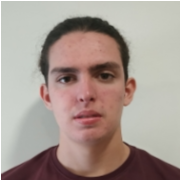
\includegraphics[width=0.15\textwidth]{imagens/fotos/A97363.png}
       \end{tabular}

       \vfill
       \vspace{0.3cm}
        \large
       Grupo 7 \\
       \href{https://github.com/dium-li3/grupo-07}{https://github.com/dium-li3/grupo-07} \\
       \vspace{0.8cm}
       
       \begin{center}
           
\includegraphics[width=0.3\textwidth]{imagens/capa/um.png}
       \end{center}
       
       \normalsize
       %\includegraphics[width=0.4\textwidth]{university}
       Departamento de Informática\\
       Universidade do Minho\\
       Janeiro 2023
            
   \end{center}
   
\end{titlepage}

\renewcommand{\contentsname}{Índice}

\tableofcontents

\pagebreak

\section{Resumo}
    \par Este relatorio diz respeito a ultima fase (II) do projeto de Laboratorios de Informatica III e tem como objetivo mostrar as metas e formas de resoluçao dos exercicios propostos e tambem as dificuldades encontradas nestes.
    \par Em comparação com a fase anterior anterior podemos dizer que esta foi bastante mais complexa de se realizar e consequentemente mais motivadora, porém foram encontrados alguns problemas na mesma. Explorou a nossa criatividade e capacidade de superar dificuldades o que nos levou a descobrir aspetos da linguagem C e de programação no geral que nunca imaginavamos.

\clearpage

\section{Avanços relativos à Fase I}

    \par Após a apresentação da I fase, a nossa realidade relativamente ao estado do nosso projeto alterou. Como futuros profissionais vimos este acontecimento como um fator muito importante para o desenvolvimento constante do nosso trabalho, acreditamos que o progresso está visível e facilmente comprovável.
    \par Começamos então por garantir o encapsulamento e modelação de todos os dados, visto que após discussões com os Docentes concluímos facilmente que este era o fator mais decisivo. Seguindo este objetivo, alteramos a arquitetura inicial da aplicação relativamente à criação das \textit{hashtables}, que se sustentava num ficheiro que continha as três principais estruturas deste projeto, passando agora a ser composta por um ficheiro para cada uma delas.
    \par Corrigimos também os problemas que tinham sido apontados na nossa Makefile.
    \par Um outro avanço relativamente à primeira fase de entrega centra-se no encapsulamento das \textit{hashtables} visto que estas eram tornadas acessíveis em outros ficheiros que não o da sua criação através do uso da primitiva \textit{\textbf{extern}} o que compromete o encapsulamento das mesmas. Face a este problema as hashtables passaram as ser criadas no ficheiro \textit{interpreter.c} onde são posteriormente acessadas nos diferentes ficheiros sendo passadas como argumentos das funcões que as invocam.
    \par Adotamos também uma nova forma de calcular campos que são frequentemente necessários/pedidos. Fazemos então o parsing dos users e dos drivers e posteriormente ao longo do parse das rides guardamos no user e driver respetivo dados como a avaliação total, o total gasto/auferido, a distância total, o número de viagens, a avaliação média, e a última ride realizada. Anteriormente a esta implementação, a informação pedida por cada querie era calculada ao longo da realização da mesma, deste modo apenas precisamos de a pedir. A implementação desta estratégia contribuiu para um melhor desempenho do programa reduzindo o tempo de execução de queries mais simples como a querie 1 e 4, por exemplo, visto que todos os dados referentes às mesmas já se encontram cálculados e guardados de antemão.
    
 \clearpage
 
\section{Modularização e reutilização de código}
    \par Modularização e reutilização de código são conceitos fundamentais no desenvolvimento de software. A modularização consiste em dividir o código em módulos separados, cada um com uma função específica e bem definida. Isso torna o código mais fácil de ser entendido, mantido e testado. Além disso, permite a reutilização de módulos em projetos futuros, economizando tempo e esforço.

    \par A reutilização de código se refere ao uso de módulos já existentes em vez de escrever novamente o mesmo código. Isso não só poupa tempo, mas também garante que o código já testado e confiável seja utilizado. Além disso, a reutilização de código pode ajudar a manter a consistência em projetos maiores e mais complexos.

    \par Ao longo do desenvolvimento deste projeto foi sempre dado o devido cuidado à manutenção da modularização e reutilização do código havendo ainda espaço para possíveis melhorias no futuro, como por exemplo, a criação de um módulo específico ao parsing de dados, contrário ao utilizado no nosso programa onde o parsing de cada ficheiro \textit{csv} é realizado no ficheiro da estrutura respetiva.
 
\section{Encapsulamento e abstração}
    \par Como referido nos \textit{Avanços relativos à Fase I}, tomamos em consideração as observações dos Docentes, pelo que modificamos no seu todo o método de encapsulamento e abstração dos dados.
    \par Primeiramente tínhamos o parsing dos catálogos concetrado num só ficheiro, tal como a criação das tabelas. Acedíamos às tabelas e ao conteúdo desejado de forma direta, ou seja, não tínhamos controlo algum sobre os dados que estavam a ser manipulados.
    \par Tivemos então de criar os ficheiros \textit{users.c}, \textit{drivers.c} e \textit{rides.c} para parsing dos dados e posterior criação das \textit{hashtables}. Fizemos funções \textit{get} e \textit{set}, que nos permitem aceder e alterar, respetivamente, os dados desejados em cada \textit{value} das tabelas. Deste modo, temos total controlo sobre aquilo que pode ou não ser acedido a partir de uma determinada zona.

 
\section{Estruturas de dados utilizadas}

    \par Devido ao facto de ser livre o uso da biblioteca \textit{glib2} utilizamos as \textit{HashTables} e as \textit{Listas} que esta biblioteca nos proporciona. Optamos por esta solução, e não pela criação das nossas próprias tabelas, pois sabiamos de antemão que estas estrututas eram bastante mais eficientes (tanto a procura por \textit{keys}, como a inserção de novos elementos). 
    

\clearpage
\section{Exercícios e Resolução}
\subsection{Parsing de dados/Validação de campos}
    O parsing de dados evoluiu um pouco ainda que a base estabelecida no final da primeira fase persistisse. O parsing, que estava até então confinado ao ficheiro \textit{main.c} onde eram criados todos os catálogos passou agora a estar disperso pelos diferentes ficheiros correspondentes a cada catálogo. Isto veio com a necessidade de uma melhoria do encapsulamento e modularização do código até então desenvolvido. Desta forma o parsing de cada ficheiro é efetuado num ficheiro próprio e, aquando do parsing do ficheiro das \textit{rides}, passaram a ser também calculados alguns valores importantes às queries.
    A validação dos campos não ficou implementada a 100\% visto que as validações dos campos \textit{\textbf{car class}} da estrutura \textit{driver} e \textit{\textbf{Acc status}} da estrutura \textit{user}
    inválidos acabam por passar na validação ainda que erroneamente.
    
\subsection{Querie 1}
    \par Procuramos o \textit{id/username} fornecido nas nossas tabelas e, como já temos todos os dados necessários guardados nas estruturas, basta fazermos os acessos aos dados de interesse e imprimi-los para o ficheiro de output.

\subsection{Querie 2}
    \par Primeiramente passavamos os dados da \textit{drivers table} para um array auxiliar, sendo a key o \textit{id} do driver e o value seria o \textit{driver}. Posteriormente ordenamos o array pelos parâmetros pedidos, mas não estávamos a ter sucesso. Utilizamos a função \textit{qsort} para este efeito.
    \par Vimo-nos então obrigados a mudar de estratégia. Neste momento estamos a criar uma nova tabela com os \textit{drivers} ordenados de forma correta (teoricamente, pois mesmo assim a ordenação não está a correr como o esperado).

\subsection{Querie 3}
    \par Alvo de uma estratégia similiar à querie 2, assim como todas as queries TopN (no enunciado dao outro nome). Este método acatava com \textit{leaks} de memória que alcançavam os 19MB de dados. Face a este problema optamos, posteriormente pela conversão das entradas da \textit{hashtable users} numa \textit{GList}, à qual seria feita a ordenação dos valores. Nesta fase a querie já produzia um \textit{output}, no entanto, os valores apresentados não eram os corretos, pelo que a ordenação não estava a ser realizada corretamente. Dito isto, numa última tentativa de corrigir esta querie alterada a abordagem passando a transformar a hashtable numa hashtable iterativa, ainda que, sem resultado visto que o problema pareceu persistir ao nível da função de comparação utilizada na ordenação.
    \subsection{Querie 4}
    \par Iteramos a \textit{\textbf{rides table}} com a função \textit{g\_hash\_table\_iter\_init}, da biblioteca \textit{glib}, e a cada iteração é comparada a cidade da \textit{ride} em questão com a cidade objetivo: se forém iguais, é calculado o seu preço.
    \par Neste momento precisamos de verificar qual a classe do veículo utilizado nesta viagem. Assim, basta aceder ao \textit{driver} pretendido através do seu \textit{\textbf{id}}, que o podemos obter pela viagem e verificar a classe do seu carro. Para classes e distâncias de viagens diferentes teremos custos diferentes. O preço total  e o número de viagens são guardados e atualizados a cada iteração e, deste modo, é possível calcular o preço médio das viagens na cidade objetivo.

\subsection{Querie 5}
    \par Primeiramente, é efetuado o parsing das datas atribuindo cada valor a um inteiro. Em seguida, é utilizada a função \textit{g\_hash\_table\_iter\_init}, da biblioteca \textit{glib}. A cada iteração a data de cada \textit{ride} é comparada com as datas fornecidas no input da querie de modo a verificar-se se esta se encontra no intervalo de datas pretendido e no caso deste último é feito o acesso ao \textit{driver}, que corresponde ao \textit{\textbf{driver id}} da \textit{ride} acedida previamente, que se encontra na \textit{hashtable \textbf{drivers table}}. 
    \par Tendo acesso ao \textit{driver} é acedido o campo \textit{\textbf{car class}} e dependendo do tipo de carro é efetuado o cálculo do custo dessa viagem e guardado o valor num \textit{int \textbf{preco viagem}}. É também incrementada a varíavel \textit{int \textbf{n viagens}} que representa o número de viagens que se encontram no intervalo de tempo estipulado pelas datas recebidas na querie.
    \par Dado como terminadas a pesquisa das keys da \textit{\textbf{rides table}} é calculado o custo médio das viagens e guardado na varíavel \textit{int \textbf{preco medio}} sendo, por último, impresso este valor no ficheiro para o qual o caminho está contido, como dito anteriormente, no \textit{pointer \textbf{filepointer}}.
    
\subsection{Querie 6}
    \par O processo de execução desta querie é, essencialmente, o mesmo da querie5, com a pequena excessão de que, aquando da validação que permite averiguar se a data de uma \textit{ride} se encontra no intervalo de tempo fornecido na querie é também verificada em simultâneo se a cidade onde a \textit{ride} em questão foi providenciada é a mesma do que a cidade que fora fornecida previamente como argumento da querie.
    Após esta verificação o processo de execução toma um rumo similar ao da querie5 novamente.
\subsection{Querie 7}
    \par A estratégia utilizada para este exercício é muito similar à da \textit{querie 2}, a pequena diferença é o uso de uma tabela auxiliar para guardar todas os \textit{drivers} que satisfaçam os requisitos.
    \par A partir desta tabela criamos uma nova tabela ordenada (teoricamente), consoante os parâmetros pedidos, com as \textit{rides} desejadas.
    
\subsection{Querie 8}
    \par Estrutura bastante similar à \textit{querie 7}, mas guardamos as \textit{rides} desejadas numa nova tabela para depois ser possível ordenar. Visto que tivemos um problema com as funções de ordenação e, como o nosso tempo já não era muito, optamos por dar prioridade a outros pontos do projeto.
    
\subsection{Querie 9}
    \par A implementação elaborada para esta querie é muito similar à querie 5, cada \textit{ride} que verifique a condição estabelecida, onde a \textit{\textbf{data}} da ride se encontra no intervalo estabelecido pelo \textit{input} da querie e o cliente deu gorjeta, é adicionada à tabela auxiliar.
    \par Esta tabela posteriormente dá origem a uma outra ordenada (teoricamente), com as \textit{rides} desejadas. Visto que tivemos um problema com as funções de ordenação e, como o nosso tempo já não era muito, optamos por dar prioridade a outros pontos do projeto. 
\clearpage

\section{Interface}
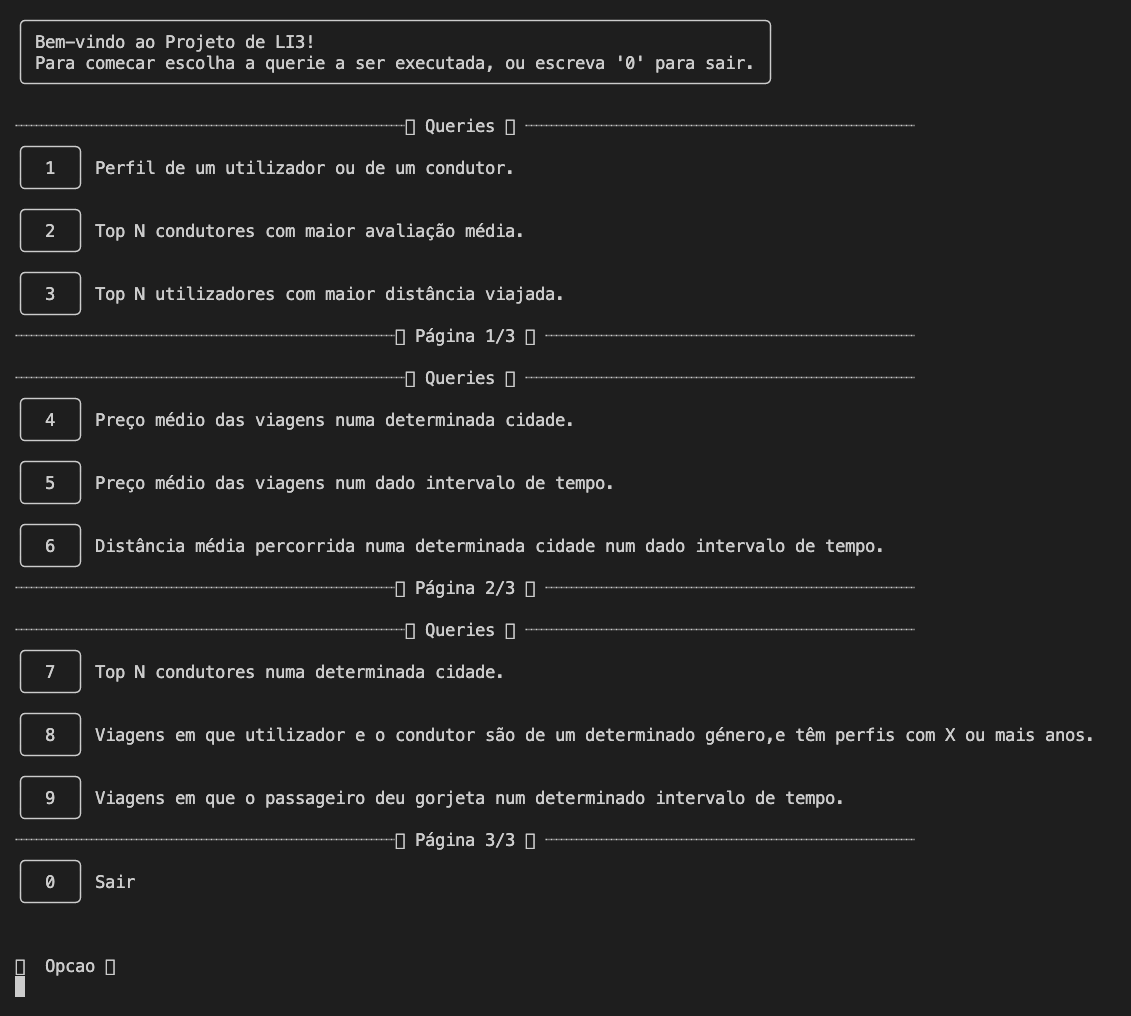
\includegraphics[width=1\textwidth]{imagens/fotos/Interface.png}

\clearpage

\section{Conclusão}
    \par Finalizando, apesar das adversidades encontradas aquando da realização do projeto, tendo em conta o volume de trabalhos que os integrantes desta equipa se encontravam envolvidos, consideramos que conseguimos atingir a maior parte dos objetivos propostos.

    \par  Ainda assim um dos objetivos cruciais para a resolução dos exercícios de top N não ficou totalmente concluído, ficando a faltar a ordenação dos \textit{outputs}. As funções de ordenação estão implementadas e sofreram uma exausta análise não tendo sido, no entanto, encontrado o erro, apesar das diferentes estratégias adotadas - entre as quais, passar todos os dados das tabelas para um array auxiliar e posteriormente ordenar utilizando a função \textit{qsort}.
    
    \par O processo de aprendizagem sobre a utilização da biblioteca GLib  é demorado e algo complexo, assim como a utilização das listas e tabelas de hash da mesma.

    
\clearpage


\clearpage

\end{document}